\documentclass{standalone}
\usepackage{tikz}
\usetikzlibrary{positioning}
\usetikzlibrary{fit}

\begin{document}

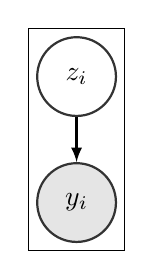
\begin{tikzpicture}
  \tikzstyle{random}=[
      circle, minimum size = 10mm, thick
    , draw = black!80
    , node distance = 16mm
    ]
  \tikzstyle{observed}=[
      circle, minimum size = 10mm, thick
    , draw = black!80, fill = black!10
    , node distance = 16mm
    ]
  \tikzstyle{connect}=[-latex, thick]
  \tikzstyle{plate}=[rectangle, draw = black!100]

  \node[random] (z) { $z_{i}$ };
  \node[observed] (y) [below of = z] { $y_{i}$ };

  \path (z) edge [connect] (y);

  \node[plate, inner sep = 1.0mm, fit = (z) (y)] { };

\end{tikzpicture}

\end{document}
